\documentclass{beamer}
\usepackage{hyperref}
\usepackage{caption}
\usepackage{sagetex}
\hypersetup{
	colorlinks=true,
	linkcolor=blue,
	urlcolor=blue,
}
\setbeamercolor{note page}{bg=white}
\usepackage{wrapfig}
\usepackage{blindtext}
\usepackage{pythontex}
\usetheme{Warsaw} % This line sets the theme
\usecolortheme{beaver}
\setbeameroption{hide notes}
\definecolor{dkgreen}{rgb}{0,0.6,0}

\newcounter{slidenum}
\usepackage{xcolor}
\definecolor{mauve}{rgb}{0.58,0,0.82}

\usepackage{listings}

\lstset{
	language=Python,                 % the language of the code
	basicstyle=\tiny\ttfamily,       % the size of the fonts that are used for the code
	numbers=left,                    % where to put the line-numbers
	numberstyle=\tiny\color{gray},   % the style that is used for the line-numbers
	stepnumber=1,                    % the step between two line-numbers. If it's 1, each line will be numbered
	numbersep=5pt,                   % how far the line-numbers are from the code
	backgroundcolor=\color{white},   % choose the background color. You must add \usepackage{color}
	showspaces=false,                % show spaces adding particular underscores
	showstringspaces=false,          % underline spaces within strings
	showtabs=false,                  % show tabs within strings adding particular underscores
	frame=single,                    % adds a frame around the code
	rulecolor=\color{black},         % if not set, the frame-color may be changed on line-breaks within not-black text (e.g. comments (green here))
	tabsize=2,                       % sets default tabsize to 2 spaces
	captionpos=b,                    % sets the caption-position to bottom
	breaklines=true,                 % sets automatic line breaking
	breakatwhitespace=false,         % sets if automatic breaks should only happen at whitespace
	title=\lstname,                  % show the filename of files included with \lstinputlisting; also try caption instead of title
	keywordstyle=\color{blue},       % keyword style
	commentstyle=\color{dkgreen},    % comment style
	stringstyle=\color{mauve},       % string literal style
	escapeinside={\%*}{*)},          % if you want to add LaTeX within your code
	morekeywords={*,...}             % if you want to add more keywords to the set
}


\usepackage[utf8]{inputenc}
\usepackage[T1]{fontenc}
\usepackage{graphicx}

\title{Linear Regression in Python}
\author{Jose Chavez}
\date{\today}

\titlegraphic{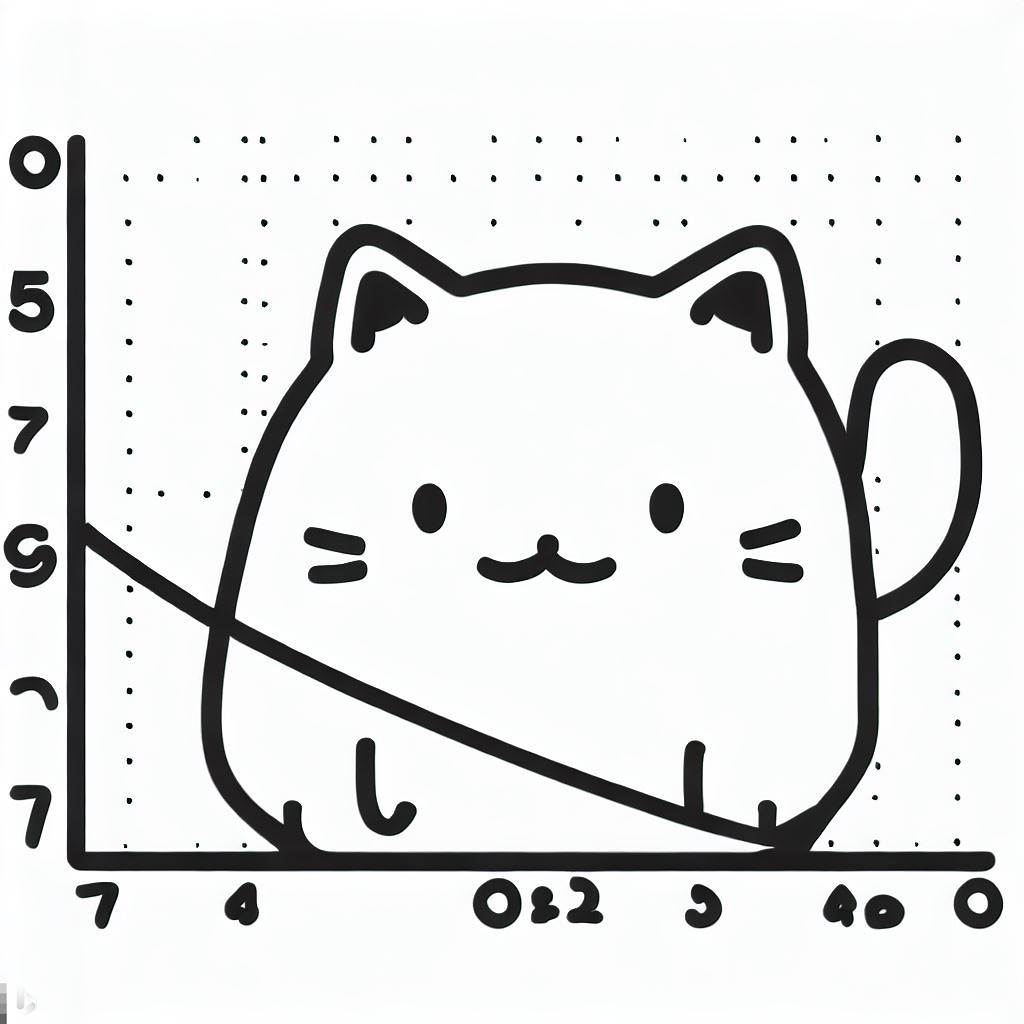
\includegraphics[width=3cm]{catLG.jpeg}}

\setbeamertemplate{footline}
{
	\hbox{%
		\begin{beamercolorbox}[wd=.4\paperwidth,ht=2.25ex,dp=1ex,center]{author in head/foot}%
			\usebeamerfont{author in head/foot}\insertshortauthor
		\end{beamercolorbox}%
		\begin{beamercolorbox}[wd=.6\paperwidth,ht=2.25ex,dp=1ex,center]{title in head/foot}%
			\usebeamerfont{title in head/foot}\insertshorttitle\hspace*{3em}
			\insertframenumber{} / \inserttotalframenumber\hspace*{1ex}
	\end{beamercolorbox}}%
	\vskip0pt%
}

\begin{document}

\frame{\titlepage}

\begin{frame}
	\stepcounter{slidenum}
\frametitle{Table of Contents}
\tableofcontents
\end{frame}


\begin{frame}
	\stepcounter{slidenum}
\section{Introduction}
\frametitle{Recap and Introduction}
\begin{itemize}
\item Linear Regressions: 
	Dependent variable ($y$) and one or more independent variables ($x_1, x_2, ..., x_n$).\\
	Fitting a linear equation to the observed data. \\
	Minimize differences between. real and predicted

The linear regression model is represented by the equation:

\[ y = b_0 + b_1x_1 + b_2x_2 + ... + b_nx_n \]
where:
\begin{itemize}
    \item $y$ is the dependent variable (the one we want to predict),
    \item $b_0$ is the intercept (the value of $y$ when all $x$ values are zero),
    \item $b_1, b_2, ..., b_n$ are the coefficients (slope) for each independent variable $x_1, x_2, ..., x_n$.
\end{itemize}
\item Simple yet instructive case\ldots good old
	$ y = mx + b$

\end{itemize}
\stepcounter{slidenum}
\note{ \arabic{slidenum} Hi class. How are you all doing? Recall that last class we covered the
main concepts behind linear regression and we saw a simple example with ages
and heights as features. I promised that today we would see how to do all of
this with Python. 
}
\end{frame}

\begin{frame}
	\frametitle{Hypothetical Project}
\stepcounter{slidenum}
	\note{let's assume that we are being asked to find a relationship between the age of twitter
	users and their average rate, per week of twitter usage. We suspect that there's probably
some relationship, in fact its probably safe to say that most people would expect older users to
tweet less often, right? Let's get a feel for that. }

	Question:\\
	Are older Twitters user's less likely to use the app throughout the week? What's the
	relationship between age usage? 

\end{frame}


\begin{frame}
\section{Data Set: Fake Twitter Data}
\frametitle{Data: Fake Twitter Data}
\stepcounter{slidenum}
\note{Let's talk about what data we're going to be using. I took the liberty of
dveloping some python scripts that generate three years of ``fake data'' for a
database of twitter users. I used Poissson distributions and an assortment of
custom scripts to simulate many records. You can find the scripts and
colloborate with me potentially on them by visiting the link provided.

Now imagine this. You are a data scientist with access to an api providing the
data in csv format and are being asked to quickly establish some sort of
usable mathematical relationship between user age and the amount that they
tweet per week.


Now the data that we are going to be working with was created by me via Python. 
It's fairly simple. It's a essentially csv data consisting of two columns corresponding to age and
average number of tweets per week. You can find the code used to generate it as well as some more
flexible but complex code at the github link provided in our slides. 

I didn't use real data because the real data available from twitter online doesn't contain any user
information to protect privacy not even ages. I wanted to demonstrate something to do with age so
decided to take the liberty. 
}%end for note
\begin{columns}
\column{0.5\textwidth}
{\scriptsize
\begin{itemize}
	\item Hypothetical Data Scientist scenario: \\
		You are asked to investigate the connection between age and
		tweet rates.

		You are given an access token to an API.

	\item Dataset for our demonstration: Python scripts you can find at: 
		\href{https://github.com/jgcblue/lectureDS.git}{github}
		were used to generate hundreds of records of consisting of
		records that include: age, date, tweet (a string);
	\item Why not the real thing?\\
		Privacy: Twitter does not realease even that user information. 
\end{itemize}
}
\column{0.5\textwidth}
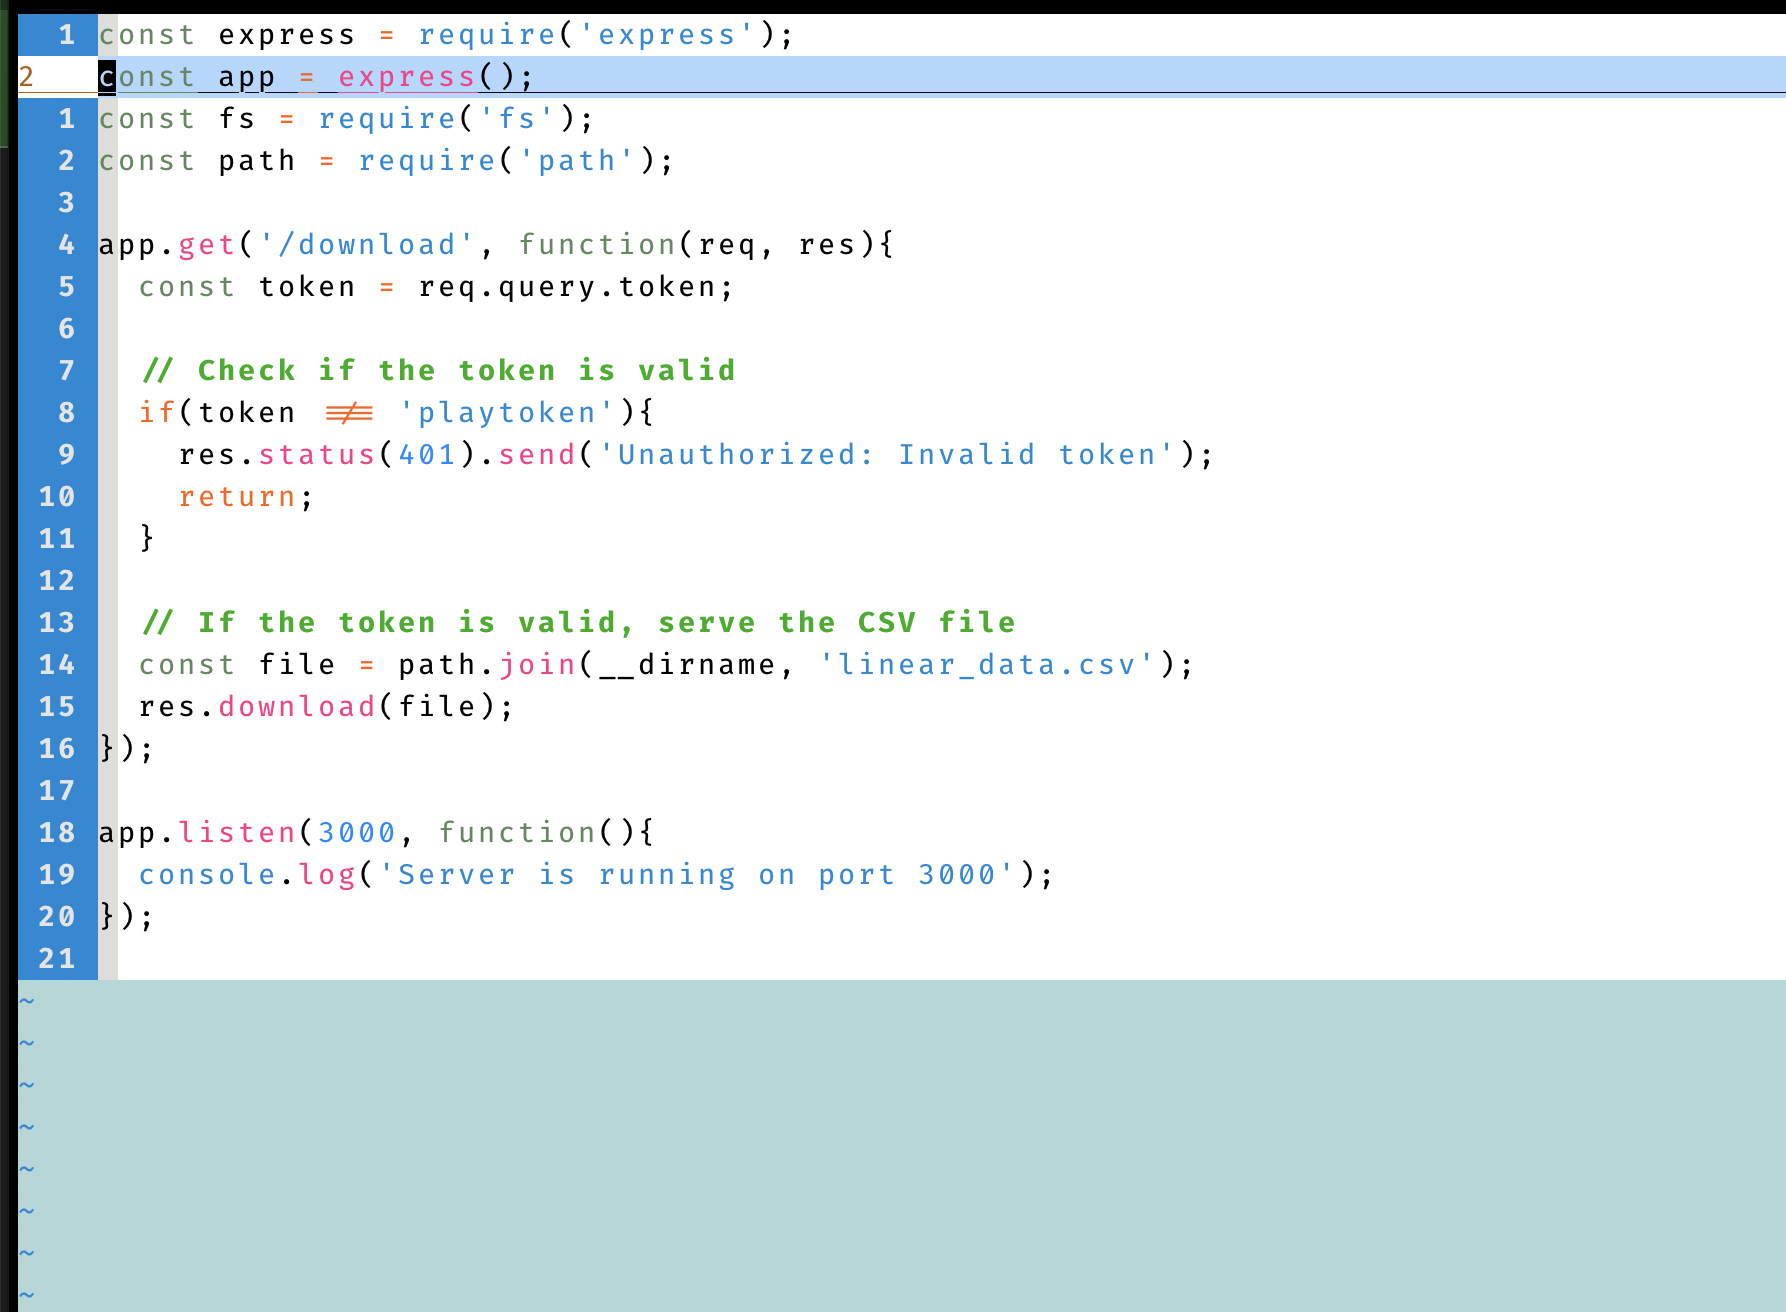
\includegraphics[width=\textwidth]{server.png}
%insert image of the api code
\end{columns}
\end{frame}

\begin{frame}
	\frametitle{The Data Science Process}
	\stepcounter{slidenum}
	\note{Before we move on, let's remember to }
	\begin{itemize}
	\item \textbf{Understand the Problem:} Define problem and objective.\\

		Here: The problem is finding a relationship between the ages
		and weekly tweet rates.
  \item \textbf{Data Collection:} Gather data.\\
  \item \textbf{Exploratory Data Analysis (EDA):} Explore the data to get a
	  feel for its strucute. \\
	  Here: We're going to view a scatter plot to get a rough idea whether
	  or not we should expect any success.
\end{itemize}
\end{frame}

\begin{frame}{The Data Science Processs (2)}
	\stepcounter{slidenum}
	\note{Page: \thepage Continuing on we need to choose features, recall that this is the
	part of the data that we choose to potentially explain what we're
interested in. In this case we're interested in the rate of tweets and we only
have one features so our task is simple this time. }
	\begin{itemize}	
  \item \textbf{Feature Selection:} Choosing relevant features (given in our
	  problem).\\

	  Here: This is straighforward in our scenario. 
  \item \textbf{Data Splitting:} split to train and to test.
	  \note{We will use Python to split the set. More on that when we get
	  there.}

  \item \textbf{Model Building:} Use data to create a model. 
  \note[item]{If this was last week we'd be doing the linear regression ourselves. This morning we will be using python's scikit-learn library.}
  \item \textbf{Model Evaluation:} Assess the model's performance using evaluation metrics like Mean Squared Error (MSE), R-squared, or Root Mean Squared Error (RMSE).
	  \note{We are again going to benefit from Python when it comes to this
	  but we will have use our knowledge to interpret the values.\thepage}
	  \end{itemize}
\end{frame}

\begin{frame}
	
	\frametitle{The Data Science Process(3)}
	\stepcounter{slidenum}
	{\small
	\begin{itemize}
		
  \item \textbf{Model Validation:} Validate the final model on the testing data to ensure it generalizes well to new, unseen data.

  \item \textbf{Interpretation:} Interpret your findings. 

  \item \textbf{Deployment:} Deploy the trained model to make predictions on new data or integrate it into a larger application.

 \item \textbf{Monitoring and Maintenance:} Monitor the model's performance, retrain, tune, etc.
\end{itemize}
}
\end{frame}


\begin{frame}
\section{Python and Linear Regression}
\stepcounter{slidenum}
\frametitle{Python and Linear Regression}
\begin{itemize}
\item Idea: Use Python's linear regression library
\item Python Libraries:
	\begin{enumerate}
		\item [] Importing and cleaning the data:
			\begin{itemize}
				\item pandas: data structures to hydrate;

				\item python scripts for detecting and removing
					outliers and null values;
			\end{itemize}
		\item [] Exploring the data:
			\begin{itemize}
				\item matplotlib 
			\end{itemize}
		\item [] Model training and evaluation: 
			\begin{itemize}
		\item \lstinline{import sklearn as sk}
				\item sk.LinearRegression;
				\item 
			\end{itemize}
		\item [] Visualing the model's results
		\item matplotlib
	\end{enumerate}
\end{itemize}
\end{frame}

\begin{pycode}
import pandas as pd
# Assuming you have a CSV file named 'data.csv' in the same directory
df = pd.read_csv('../pe/dlc/linear_data.csv')
limited_df = df.head(7)
# Convert the DataFrame to a LaTeX table and save it as a string
latex_table = limited_df.to_latex(index=False)
\end{pycode}

\section{An Example}
\subsection{Data Collection}
\begin{frame}[fragile]
	\stepcounter{slidenum}
	\frametitle{Collect Data from our API}
	\begin{columns}
\column{0.5\textwidth}
How does text interact with this.
Our training data we set aside seems to ``align'' with the line\ldots
\column{0.5\textwidth}
\py{latex_table}

\end{columns}

	\note{Let' assume that we have a token and get access to our twitter data and that it looks
	something like what's shown. Again the idea is that you would use your token and access the
API endpoint which would in turn send you the csv. Now we need to hydrate a python object that lets
us work with this. In effect we want to be able to use the pandas library to clean up the data at a
minimum so that we might have data structures that can be used in tandem with the sk learn tools
we will be bringing in. }
	
\end{frame}


\begin{frame}[fragile]
	\stepcounter{slidenum}
	\frametitle{Collect Data from our API (2)}
	\begin{columns}
\column{0.5\textwidth}

The JavaScript Node.js Application serving the csv file we generated with
Python.
\column{0.5\textwidth}
\vspace{.5cm}
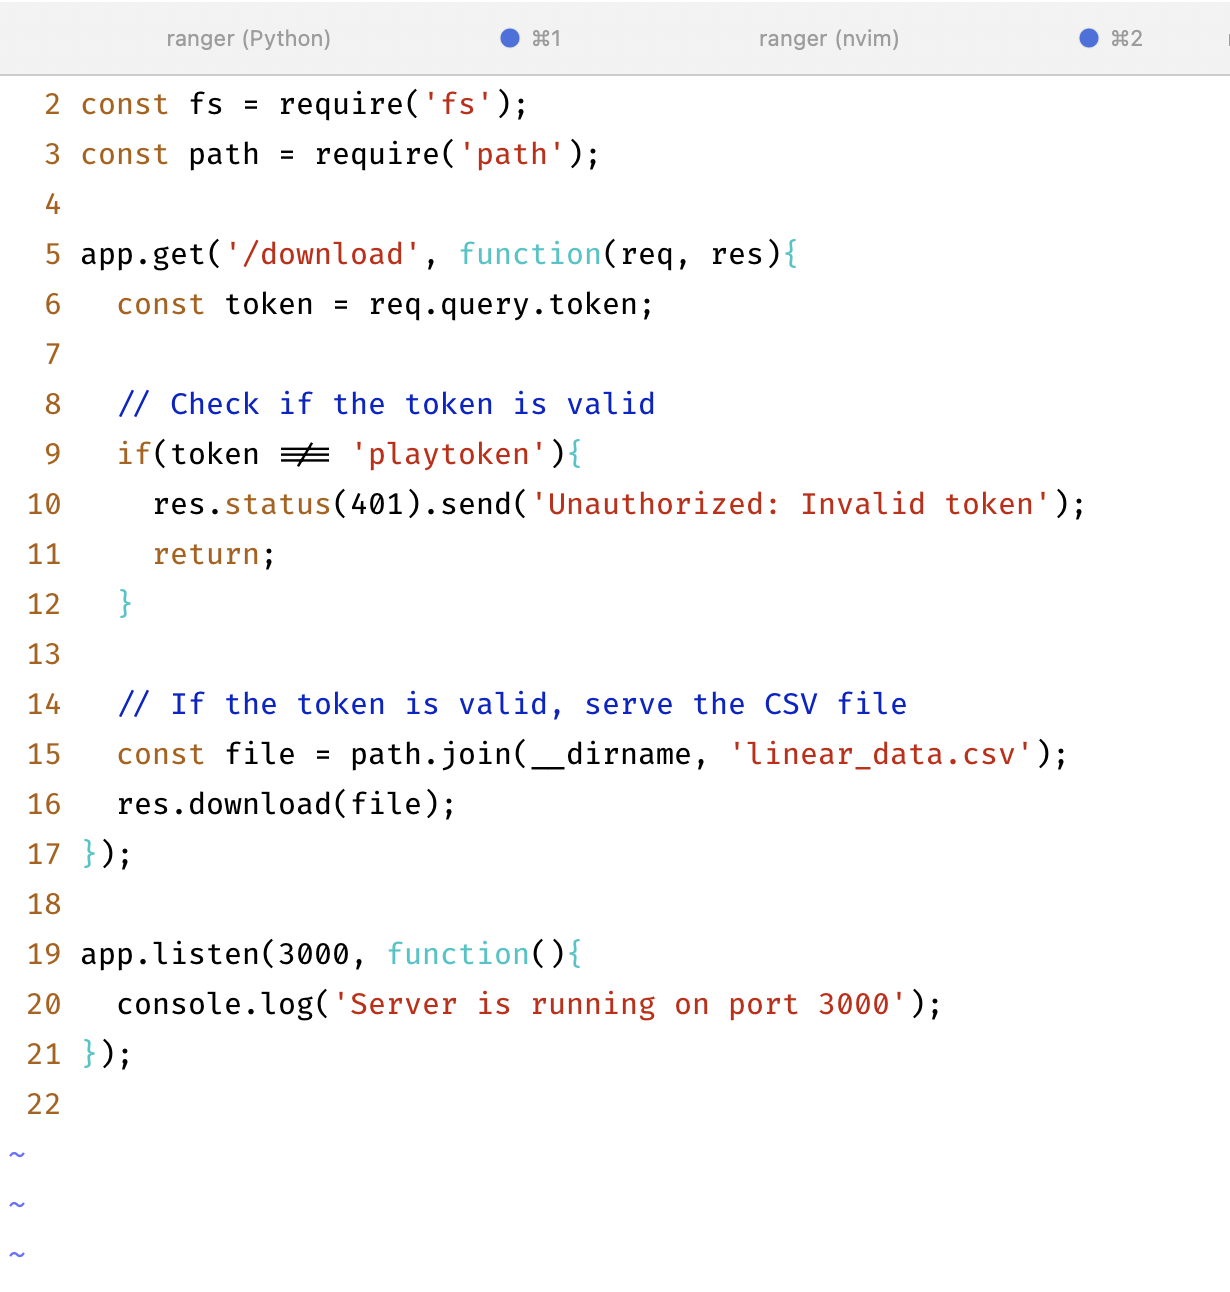
\includegraphics[height=5.5cm]{pics/server.png}
To access:
\lstinline{curl -i http://csv.bluewfjc.online/download?token=playtoken}

\end{columns}

	\note{Let' assume that we have a token and get access to our twitter data and that it looks
	something like what's shown. Again the idea is that you would use your token and access the
API endpoint which would in turn send you the csv. Now we need to hydrate a python object that lets
us work with this. In effect we want to be able to use the pandas library to clean up the data at a
minimum so that we might have data structures that can be used in tandem with the sk learn tools
we will be bringing in. }
\end{frame}

\begin{frame}[fragile]
	\stepcounter{slidenum}
	\frametitle{Hydrating a DataFrame}
	\begin{columns}

\column{0.5\textwidth}
We load the csv into a pandas DataFrame.
\column{0.5\textwidth}
	\begin{lstlisting}
import pandas as pd
df = pd.read_csv('filename.csv')
	\end{lstlisting}
\end{columns}
\end{frame}
\begin{pycode}
import seaborn as sns
import matplotlib.pyplot as plt
import pandas as pd
sns.scatterplot(data=df, x='ages', y='rates')

plt.savefig('scatter_plot.png')
\end{pycode}
\begin{frame}
	\stepcounter{slidenum}
	\frametitle{Examine Visuals of Data}

	\begin{columns}
\column{0.5\textwidth}
	Plotting ages versus rates per week
	Does it look linear? 
\column{0.5\textwidth}
	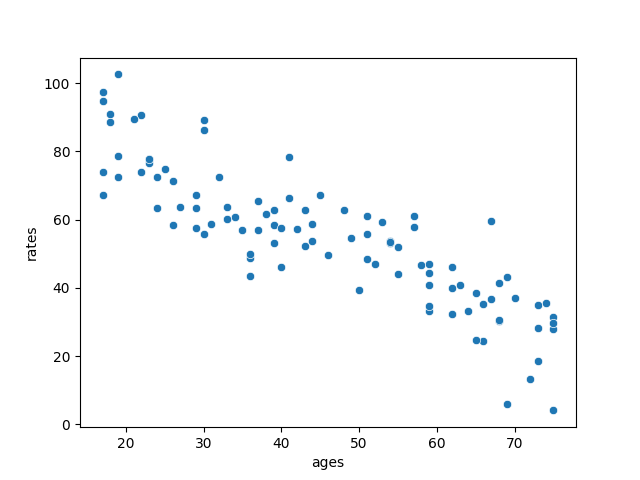
\includegraphics[width=\textwidth, height = 5cm]{scatter_plot.png}
\captionof{figure}{Scatter Plot of Data Produced with Matplotib}
\end{columns}
	
\end{frame}


\begin{pycode}
	
	# Drop negative values
df = df[df['rates'] >= 0]
# Drop null values
df = df.dropna()

# Display the first few rows of the dataframe
df.head()
Q1 = df.quantile(0.25)
Q3 = df.quantile(0.75)
IQR = Q3 - Q1

# Remove outliers
df_no_outliers = df[~((df < (Q1 - .8 * IQR)) | (df > (Q3 + .8 * IQR))).any(axis=1)]

# Display the first few rows of the dataframe without outliers
df_no_outliers.head()
# Plot ages versus rates for the original dataframe
plt.figure(figsize=(10, 5))
plt.subplot(1, 2, 1)
plt.scatter(df['ages'], df['rates'])
plt.title('Original Data')
plt.xlabel('Ages')
plt.ylabel('Rates')

# Plot ages versus rates for the dataframe without outliers
plt.subplot(1, 2, 2)
plt.scatter(df_no_outliers['ages'], df_no_outliers['rates'])
plt.title('Data Without Outliers')
plt.xlabel('Ages')
plt.ylabel('Rates')

plt.tight_layout()
plt.savefig('scatter_plots2.png')  # Save the scatter plots
plt.close()

# Box and whisker plots
plt.figure(figsize=(10, 5))
plt.subplot(1, 2, 1)
df.boxplot(column=['rates'])
plt.title('Original Data')

plt.subplot(1, 2, 2)
df_no_outliers.boxplot(column=['rates'])
plt.title('Data Without Outliers')

plt.tight_layout()
plt.savefig('scatter_plots3.png')  # Save the scatter plots
plt.close()

	
\end{pycode}


\begin{frame}[fragile]
	\stepcounter{slidenum}
	\frametitle{Cleanup}
	\note{ \arabic{slidenum}Now if one were to examine the records in their entirety, one
		would discover that there's some negative values and some
	outliers and such. So I opted to use the IQR method to get rid of the
outliers and we used some pandas functions available on dataframes to drop null
values. This is common practice. When you see ``wild'' data you will come
accross some quite random stuff and pandas' methods really come in handy. }
	\begin{columns}
\column{0.5\textwidth}
Removes negative 'rates' values\\
\vspace{.2cm}
Drops rows with null values\\
\vspace{.2cm}
Displays initial cleaned data\\
\vspace{.2cm}
Calculates quartiles and IQR\\
\vspace{.2cm}
Removes outliers from data\\
Displays data without outliers
\column{0.5\textwidth}
	\begin{lstlisting}
	# Drop negative values
df = df[df['rates'] >= 0]
# Drop null values
df = df.dropna()

# Display the first few rows of the dataframe
df.head()
Q1 = df.quantile(0.25)
Q3 = df.quantile(0.75)
IQR = Q3 - Q1

# Remove outliers
df_no_outliers = df[~((df < (Q1 - 1.5 * IQR)) | (df > (Q3 + 1.5 * IQR))).any(axis=1)]

# Display the first few rows of the dataframe without outliers
df_no_outliers.head()
	\end{lstlisting}
\captionof{figure}{Pyt Data Scatter Plot With Line}
\end{columns}
\end{frame}

\begin{frame}[fragile]
	\stepcounter{slidenum}
	\frametitle{Clean Up}
	\begin{columns}
\column{0.5\textwidth}
	Code run and differences (post IQR Method)
\column{0.5\textwidth}
	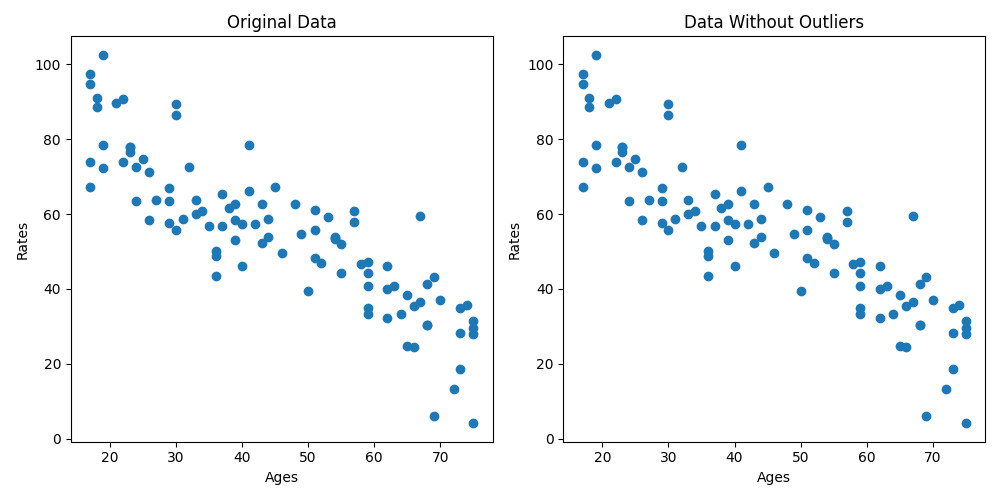
\includegraphics[height=3cm]{scatter_plots1.png}
	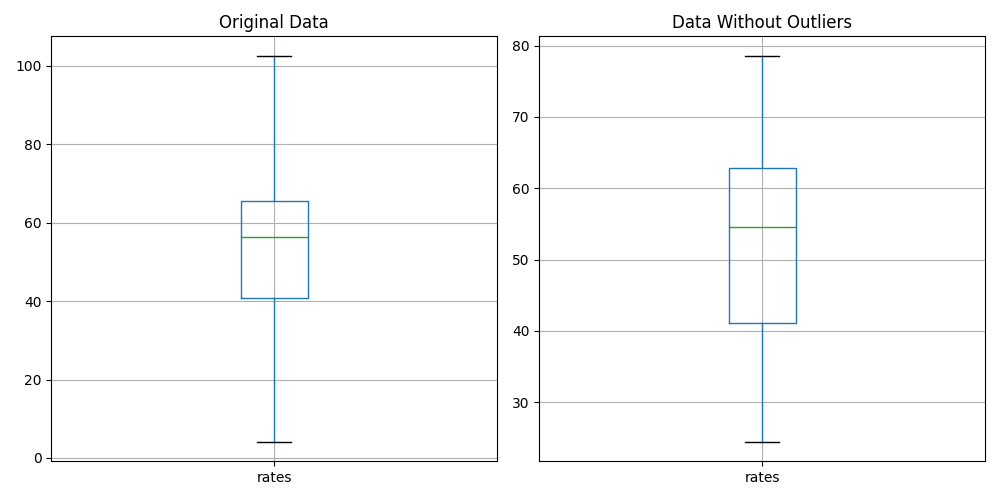
\includegraphics[height=3cm]{scatter_plots3.png}
\captionof{figure}{Box Plot Shows Outliers Have Been Extracted}
\end{columns}

	
\end{frame}

\begin{pycode}
import pickle
from sklearn.model_selection import train_test_split
from sklearn.linear_model import LinearRegression
from sklearn.metrics import mean_squared_error, r2_score
X = df_no_outliers[['ages']]
y = df_no_outliers['rates']

	# Split the data into training and test sets
X_train, X_test, y_train, y_test = train_test_split(X, y, test_size=0.2, random_state=42)

# Create a linear regression object
regr = LinearRegression()

# Train the model using the training sets
regr.fit(X_train, y_train)

# Make predictions using the testing set
y_pred = regr.predict(X_test)

# Print the coefficients
#print('Coefficients:', regr.coef_)
model_cos=regr.coef_

coefficients = regr.coef_[0]
intercept = regr.intercept_
# Print the mean squared error
#print('Mean squared error:', mean_squared_error(y_test, y_pred))
mse=mean_squared_error(y_test, y_pred)

latex_expression = f"$y = {coefficients:.2f}x + {intercept:.2f}$"

# Print the coefficient of determination (R^2 score)
#print('Coefficient of determination (R^2 score):', r2_score(y_test, y_pred))
structures_to_pickle = {
    'model': regr,
    'X_train': X_train,
    'y_train': y_train,
    'X_test': X_test,
    'y_test': y_test
}
with open('modelplus.pkl', 'wb') as file:
    pickle.dump(structures_to_pickle, file)

#r2score=r2_score(y_test,y_pred)
\end{pycode}

\begin{frame}[fragile]
	\stepcounter{slidenum}
	\frametitle{Library Imports and Splitting the Data}

	\begin{lstlisting}
from sklearn.model_selection import train_test_split
from sklearn.linear_model import LinearRegression
from sklearn.metrics import mean_squared_error, r2_score
	# Split the data into training and test sets
X_train, X_test, y_train, y_test = train_test_split(X, y, test_size=0.2, random_state=42)

# Create a linear regression object
regr = LinearRegression()

# Train the model using the training sets
regr.fit(X_train, y_train)

	\end{lstlisting}
	\note{
		{\tiny
		Okay create the model. Now we have clean data and Python is ready with its
		scikit-learn models but before we use those models we need to do an additional step
		with our data. Does anyone recall? Are we going to use all the dat? Right, so recall that first of all we need to divide our data into two
	parts. In particular we need to take a small fraction of our data and set it aside for
	testing and we are free to to use the rest for the actual training of the model. 
	So that's what you are seeing here and again this is all in our classes' python notebook so
	no worries you can find it there.
	Now I let's finally get to the exact statements and we will see that one of the lines is all
	about this splitting we just mentioned. We first see the import of sci kit learn's
	train\_test\_split split method. This method is going to help us divy up the data as we
	mentioned and I will be explaining that shortly. 
	Next we see an import of sci kit learns linearRegressio method from its linear models
	module. Recall that we access modules with packagename.module name and we add the name of a
	method if we're jsust grabbing one method. 
	Next we see that i'm importing some methods from the metrics module. In particualr tools to
	help us get the maximum error squared and r2 score. Theres are going to help us evaluate the
	model. We will also take advantage of residuals as you will see. Any questiosn? 

	Okay next we see that we are using the train\_test\_split method to actually take the data
	in and assign 20\% of the data both features and outputs as test data and the rest as
	training data. Notice the nifty destructuring going on there. The method returns four
	objects and we asign them all at once. 
	Next we instantiate an instance of a linear regression model. This is the wwhere the magic
	sort of starts right. 

	But its just a template of a linear regression model. It doesn't have any adata. 
	Well in the next line we see that we are loading the training data into th emodel and
	subsequently fitting the model. 

	Okay let's pause a moment. So we have the model now. Its parts are blackboxed for now but
	will soon see its details. 
	Before doing so let's go ahead and make some predictions. 
Recall that we divied up our data into training asets and testing sets. Its tim eto use that 20\% to
get a feel for how the model will perform. 

With that in mind we see that on line 11 we call the models predict method on the model with the
training features fed in and the 

}}.

\end{frame}

\begin{frame}[fragile]
	\stepcounter{slidenum}
	\frametitle{Gathering the Model's Parameters and Testing}
	\begin{lstlisting}[firstnumber=12]
# Make predictions using the testing set
y_pred = regr.predict(X_test)
# Print the coefficients
#print('Coefficients:', regr.coef_)
model_cos=regr.coef_

# Print the mean squared error
#print('Mean squared error:', mean_squared_error(y_test, y_pred))
mse=mean_squared_error(y_test, y_pred)

coefficients = regr.coef_[0]
intercept = regr.intercept_
# Print the coefficient of determination (R^2 score)
#print('Coefficient of determination (R^2 score):', r2_score(y_test, y_pred))
#r2score=r2_score(y_test,y_pred)
	\end{lstlisting}
\end{frame}

\begin{frame}[fragile]
	\frametitle{The Model We Have Created\ldots}
Model Coefficients:
Model Intercept (only one):

Mean Squared Error: 
	\py{model_cos}\\
	and MSE (means squared error)\\\
	\py{mse}
	\py{coefficients}\\
	and intercept \ldots\\
	\py{intercept}\\
	and as a formula:\\
	\py{latex_expression}
	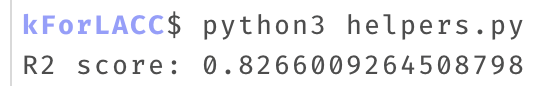
\includegraphics[width=\textwidth]{r2.png}
%coefficients = regr.coef_[0]
%intercept = regr.intercept_
\end{frame}

\begin{pycode}
plt.scatter(X_test, y_test, color='black')
plt.plot(X_test, y_pred, color='blue', linewidth=3)
plt.title('Linear Regression Model')
plt.xlabel('Ages')
plt.ylabel('Rates')
plt.savefig('plot5.png')

# Plot residuals
plt.scatter(y_pred, y_test - y_pred, color='black')
plt.hlines(y=0, xmin=y_test.min(), xmax=y_test.max(), color='blue')
plt.title('Residuals')
plt.xlabel('Predicted')
plt.ylabel('Residuals')
plt.savefig('plot6.png')
\end{pycode}
\begin{frame}
	\stepcounter{slidenum}
	\frametitle{Evaluating the Model Visually}
	\note{\arabic{slidenum} Now let's take a look at the model's
	capabilities visually. }
	\begin{columns}
\column{0.5\textwidth}
Our training data we set aside seems to ``align'' with the line\ldots

\column{0.5\textwidth}
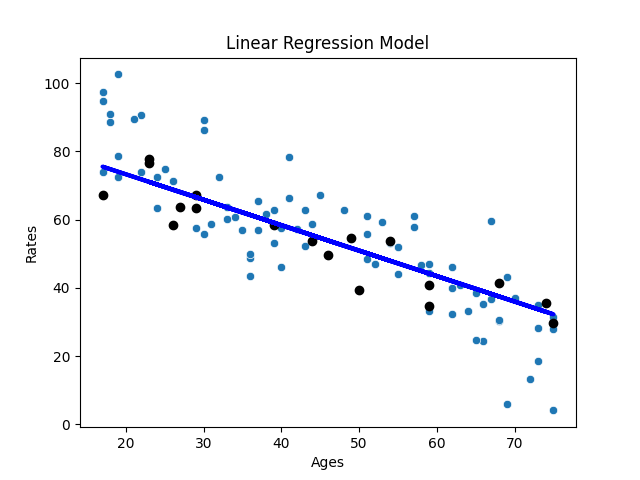
\includegraphics[width=\textwidth]{plot5.png}
\captionof{figure}{Training Data Scatter Plot With Line}
\end{columns}
\end{frame}


\end{document}

